\section{Results}

\subsection{Numerical Results}

\begin{frame}{Numerical Results}
  \setbeamertemplate{caption}[numbered]
  \begin{columns}
  \column{0.7\textwidth}
  \begin{minipage}[b][0.75\textwidth][c]{\textwidth}
\only<+>{
  \begin{figure}
  \renewcommand\thefigure{7.7} % number in thesis
  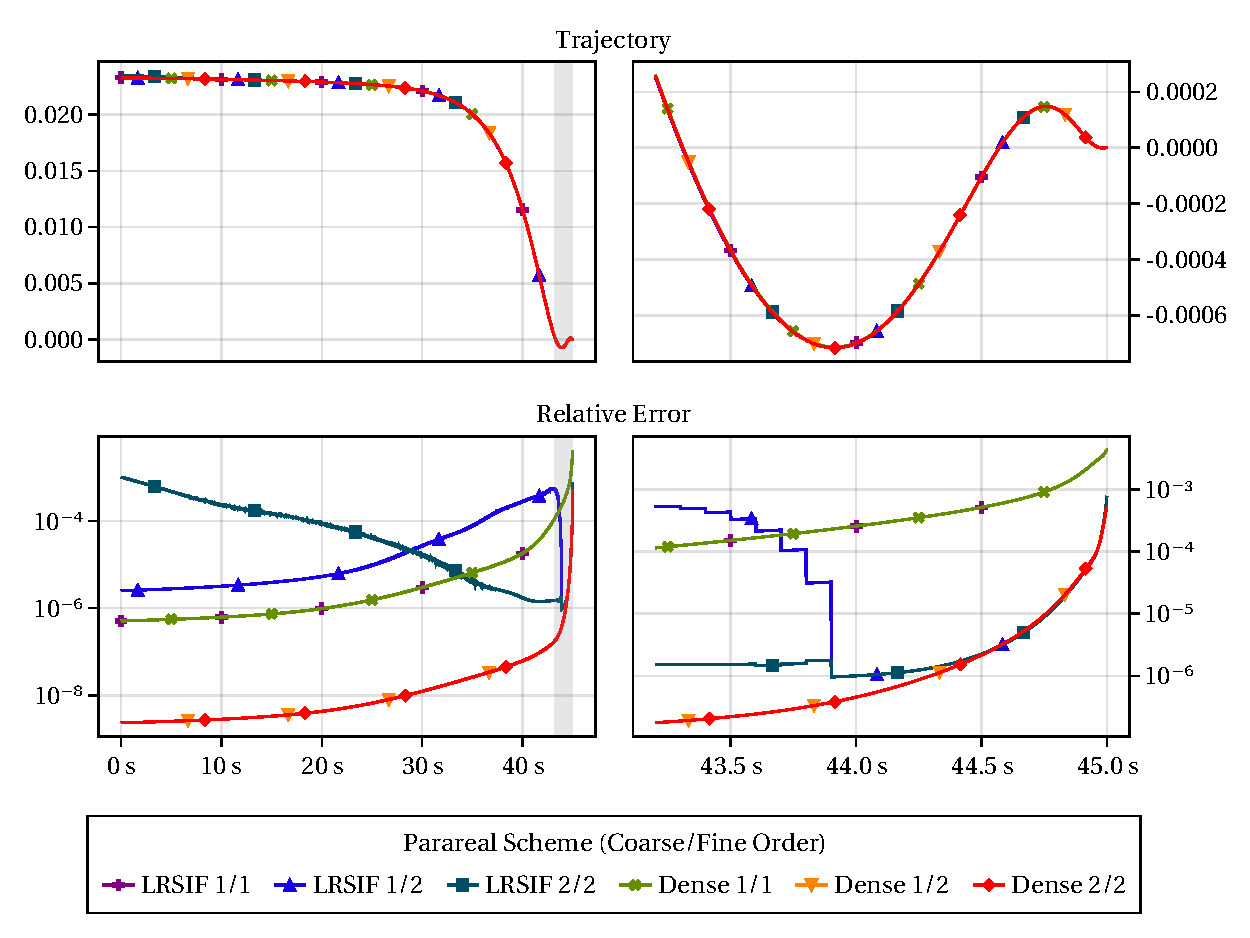
\includegraphics[width=\textwidth]{figures/fig_results_parareal.pdf}%
  \caption{Trajectory $X_{1,77}$ and relative error in $K$ for Rail371}
  \label{fig:7.7}
  \end{figure}
}
\only<+>{
  \begin{figure}
  \renewcommand\thefigure{7.8} % number in thesis
  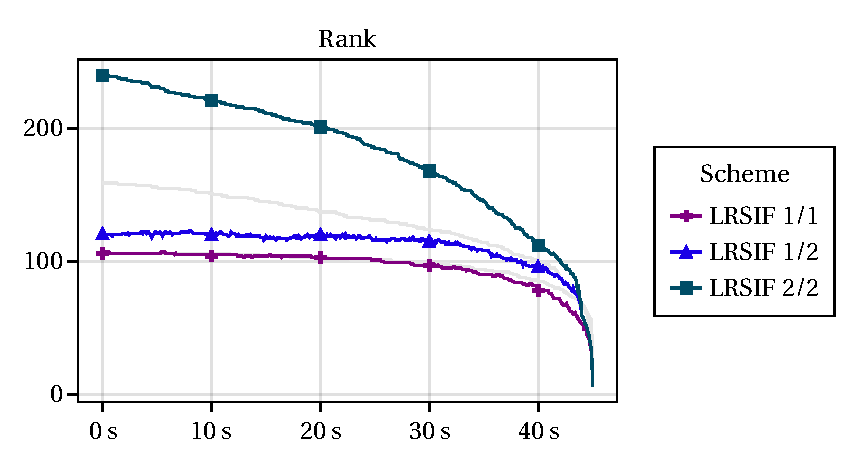
\includegraphics[width=\textwidth]{figures/fig_results_parareal_rank.pdf}%
  \caption{Rank of $X=LDL^\T$ for Rail371}
  \end{figure}
}
\only<+>{
  \begin{figure}
  \renewcommand\thefigure{7.9} % number in thesis
  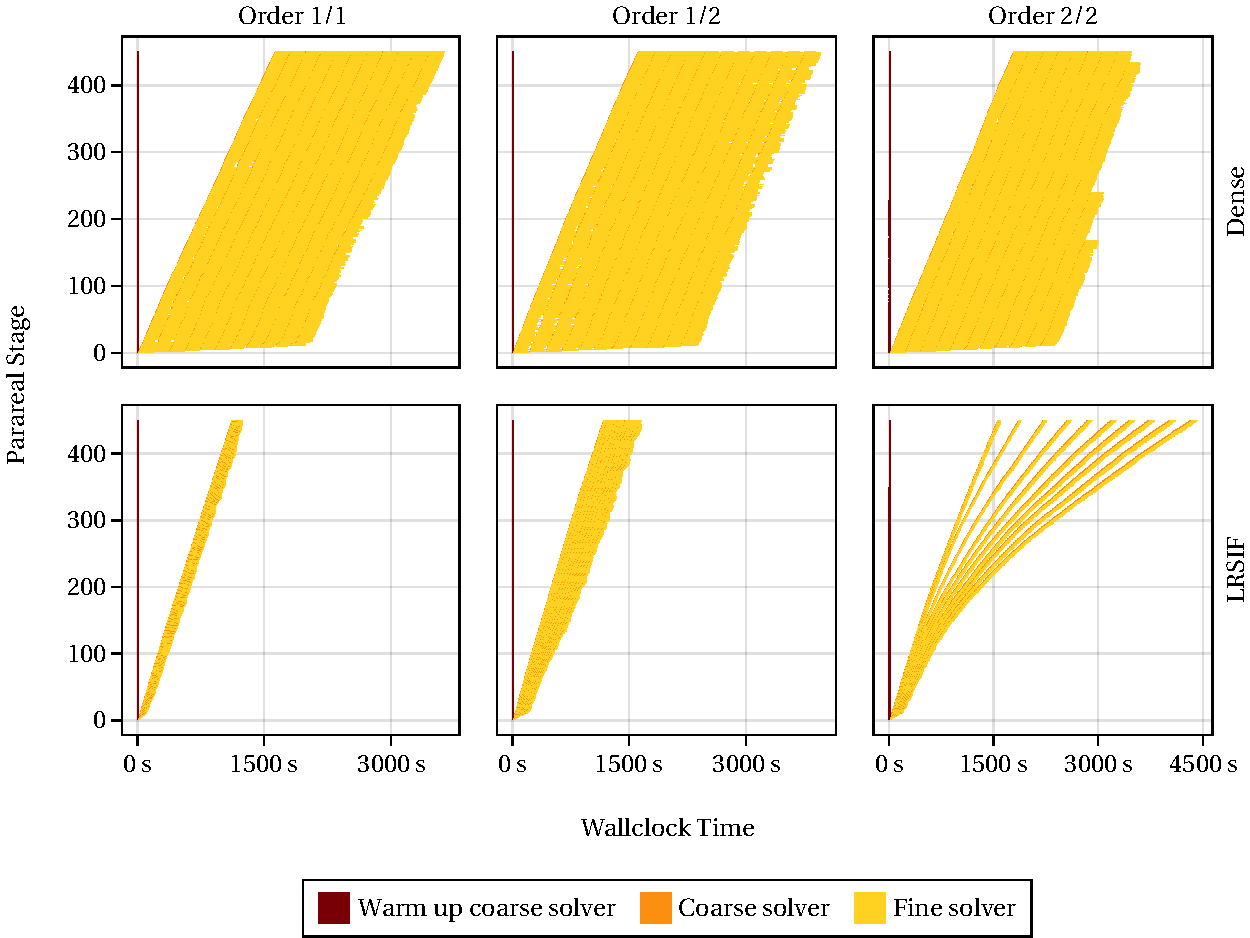
\includegraphics[width=\textwidth]{figures/fig_timeline_all.pdf}%
  \caption{Timeline chart of parareal method applied to Rail371}
  \end{figure}
}
  \end{minipage}
  \column{0.3\textwidth}
  \begin{block}{Parareal Setup}
    \begin{itemize}
      \item
        450 coarse steps (\SI{100}{\milli\second})
      \item
        100 fine steps per coarse step (\SI{1}{\milli\second})
      \item
        Maximum \#iterations: 10
      \item
        Convergence:
        relative change in~$X$\\ below $371\umach$,\\
        twice in a row,\\
        and all previous stages converged
    \end{itemize}
  \end{block}
  \end{columns}
\end{frame}

\subsection{Parallel Scaling}

\begin{frame}[b,fragile,label=speedup]{Parallel Scaling}
  \setbeamertemplate{caption}[numbered]
  \begin{columns}[c]
  \column{0.65\textwidth}
  \begin{table}
  %TODO: use hanging captions
  \renewcommand\thetable{7.3} % number in thesis
  \caption{%
    Speed-up and parallel efficiency of parareal method applied to Rail371 using $N=450$ cores.
    (timings in seconds)
  }
  \begin{tabular}{%
    l
    S[table-format=4.2] % par
    S[table-format=6.2] % seq est
    S[table-format=2.2] % speedup
    S[round-precision=3, round-minimum=0.001, table-format=1.3, table-space-text-post=$^{*}$] % efficiency
  }
    \toprule
    Solver &
    {$\tpar$} &
    {$\hattseq$} &
    {$\frac{\hattseq}{\tpar}$} &
    {$\frac{\hattseq}{N\cdot\tpar}$} \\
    \midrule
    LRSIF 1/1 & 1243.838875055313 & 4313.1015791893005 & 3.4675725816959195 & 0.007705716848213155 \\
LRSIF 1/2 & 1659.4842681884766 & 14054.911208629608 & 8.469445283727943 & 0.018820989519395426 \\
LRSIF 2/2 & 4417.833864927292 & 24565.040289878845 & 5.560426453538251 & 0.012356503230085001 \\

    \addlinespace
    Dense 1/1 & 3627.2994508743286 & 75037.70862150192 & 20.686935180776086 & 0.0459709670683913 \\
Dense 1/2 & 3956.8617849349976 & 84595.60539913177 & 21.379469386879656 & 0.04750993197084368 \\
Dense 2/2 & 3602.3622279167175 & 89274.93912768364 & 24.78233266933632 & 0.05507185037630293 \\

    \addlinespace
    Dense 4/4 & 3381.8760890960693 & 115091.05863285065 & 34.03171955469633 & 0.07562604345488073 \\

    \midrule
    \pause
    Rail1357 & 3001.4058759212494 & 22684.368317604065 & 7.557914275969537 & 0.016795365057710083$^{*}$ \\
    \bottomrule
  \end{tabular}
  \end{table}
  \column{0.35\textwidth}
  \begin{block}{Addendum}
  \begin{itemize}
    \item
      Actual runtime of (sequential) Dense 4:

      $\tseq < \SI{86831}{\second}$

      (Slurm job duration)
    \item
      LRSIF 1/1 applied to Rail1357:
      % TODO: goto button for timeline (and back button there)

      \begin{itemize}
        \item
          2 BLAS threads\\ per process
        \item
          $2\times$ round-robin scheduling onto\\
          $P=225$ processes
        \item[{\makebox[\widthof{\usebeamertemplate{itemize item}}][c]{$\ast$}}]
          actual efficiency:
          $2\hattseq/2P\cdot \tpar = \num[round-precision=3]{0.033590730115420166}$
      \end{itemize}

      % $\tpar = \SI{3600}{\second}$ (Slurm job duration)
  \end{itemize}
  \end{block}
  \hyperlink{app:rail1357}{\beamergotobutton{Appendix}}
  \end{columns}
  \onslide
  \vfill
  \begin{lstlisting}
MY_KIND=dense MY_NF=100 MY_OF=1 MY_OC=1 sbatch -n450 -J de11 par.job
  \end{lstlisting}
\end{frame}
